
\documentclass{article}
\usepackage{polski}
% \usepackage{babel}
\usepackage{amsmath} % for maths
\usepackage{graphicx} % images
\usepackage{subcaption} % subimages
\usepackage{geometry}
\geometry{
	a4paper,
	total={150mm,267mm},
	left=30mm,
	top=15mm,
}
\setcounter{section}{1} % skipping lab01

\title{Sprawozdanie nr 1\\Analiza Obrazów}
\date{2019-11-18}
\author{Tomasz Rajchel}
	
	
\begin{document}
	\maketitle
	\pagenumbering{gobble}

	\tableofcontents
	\newpage
	\pagenumbering{arabic}
	
	\section{Laboratorium 2 - Podstawowe operacje na obrazach}
	\subsection{Wstęp}
	\begin{center}
		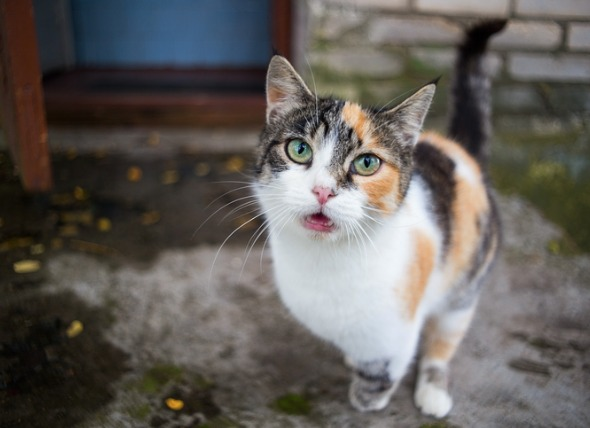
\includegraphics[width=\linewidth]{../../pictures/cat.jpg}
		\captionof{figure}{Obraz bazowy}
		\label{fig:cat}
	\end{center}
	Obraz bazowy (Rysunek \ref{fig:cat}) przekształcimy, zmieniając jego jasność, kontrast oraz luminację (korekcja gamma). Najpierw jednak zamienimy kolor z RGB na odcienie szarości.

	\begin{center}
		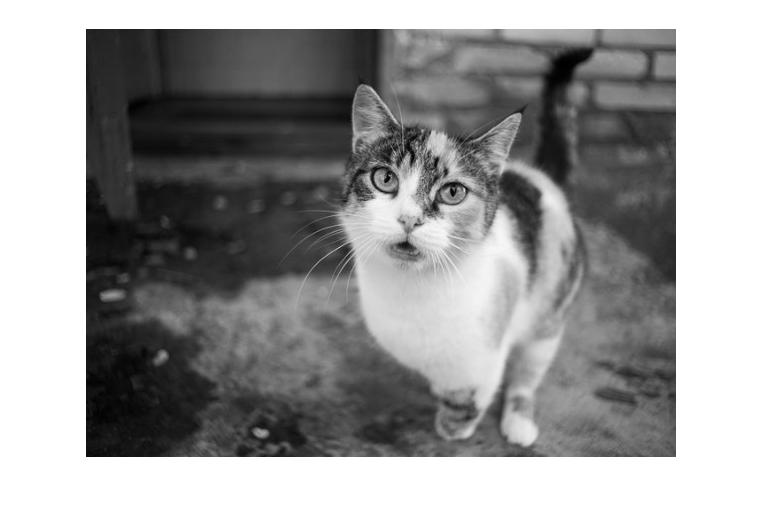
\includegraphics[width=\linewidth]{../../lab02/cat_gray.png}
		\captionof{figure}{Obraz w odcieniach szarości.}
		\label{fig:cat_gray}
	\end{center}

	\begin{center}
		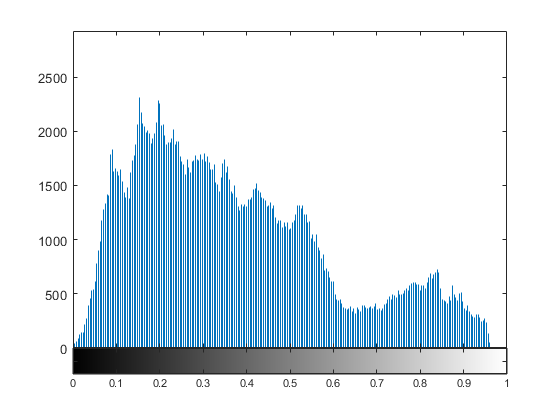
\includegraphics[width=\linewidth]{../../lab02/cat_gray_hist.png}
		\captionof{figure}{Histogram obrazu w odcieniach szarości}
		\label{fig:cat_gray_hist}
	\end{center}
	
	
	\subsection{Jasność}
	Jasność obrazu zmieniamy poprzez zwiększenie wartości każdego z pikseli. W tym przypadku do wartości każdego piksela dodajemy 0.2.
	
	\begin{center}
		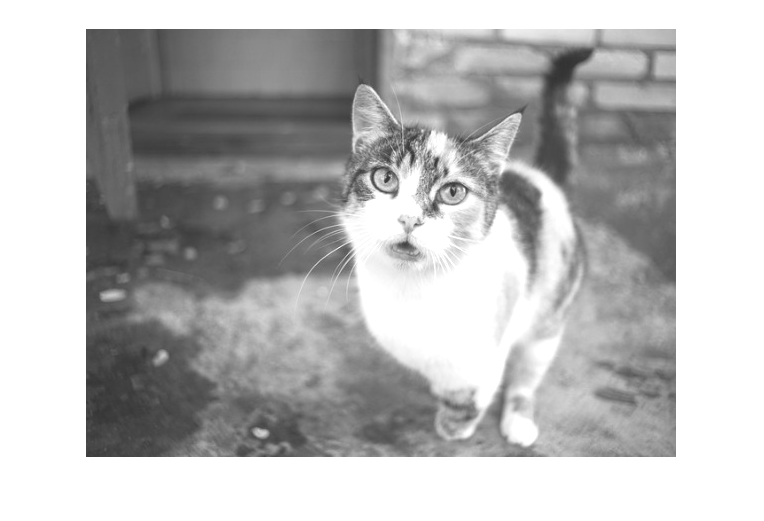
\includegraphics[width=\linewidth]{../../lab02/cat_bright.png}
		\captionof{figure}{Zwiększenie jasności}
		\label{fig:cat_bright}
	\end{center}
	
	\begin{center}
		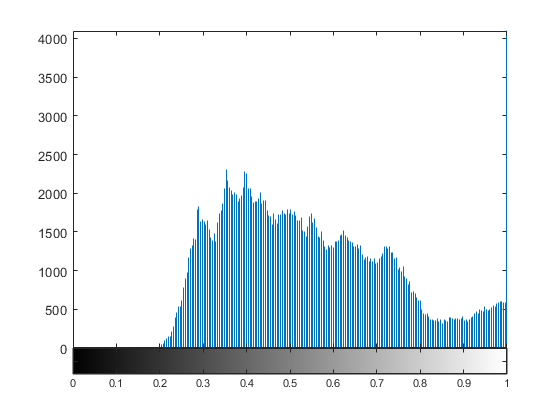
\includegraphics[width=\linewidth]{../../lab02/cat_bright_hist.png}
		\captionof{figure}{Histogram obrazu ze zwiększoną jasnością.}
		\label{fig:cat_bright_hist}
	\end{center}
	Histogram obrazu został przesunięty o 0.2 w prawo.
	
	
	\subsection{Kontrast}
	Kontrast można zmieniać poprzez pomnożenie wartości każdego piksela przez jakąś liczbe x. Poniżej przykładowe zmniejszenie kontrastu obrazu dla x = 0.5 .
	
	\begin{center}
		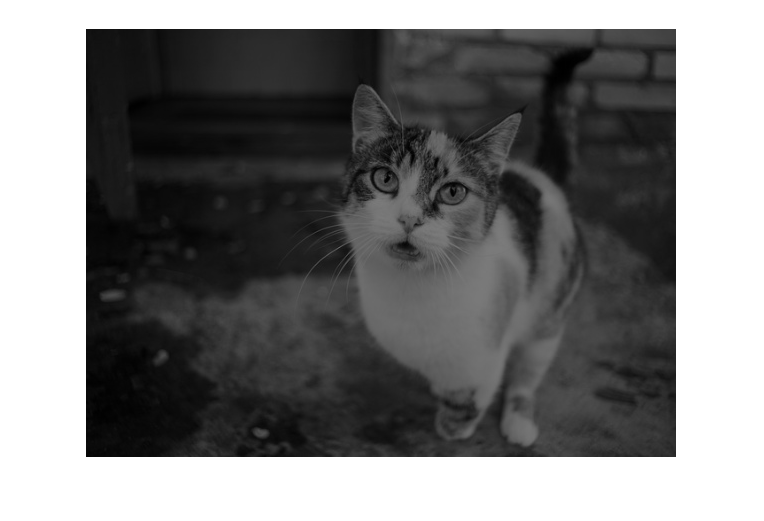
\includegraphics[width=\linewidth]{../../lab02/cat_contrast.png}
		\captionof{figure}{Zmniejszenie kontrastu}
		\label{fig:cat_contrast}
	\end{center}
	
	\begin{center}
		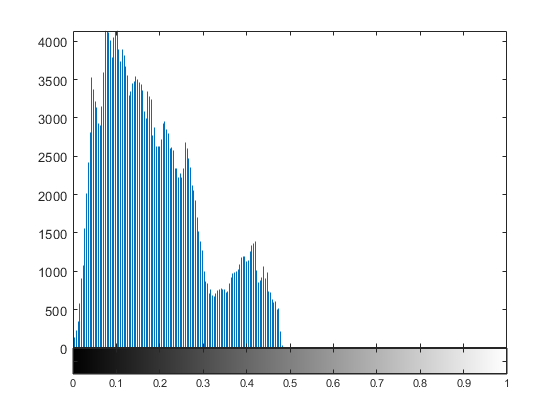
\includegraphics[width=\linewidth]{../../lab02/cat_contrast_hist.png}
		\captionof{figure}{Histogram obrazu ze zmniejszonym kontrastem.}
		\label{fig:cat_contrast_hist}
	\end{center}
	
	
	\subsection{Korekcja Gamma}
	Korekcja Gamma jest nieliniowym przekształceniem obrazu. Wartość każdego z pikseli podnosimy do potęgi $\gamma$. Poniżej przykład rozjaśniania obrazu $\gamma = 0.2$ .
	
	\begin{center}
		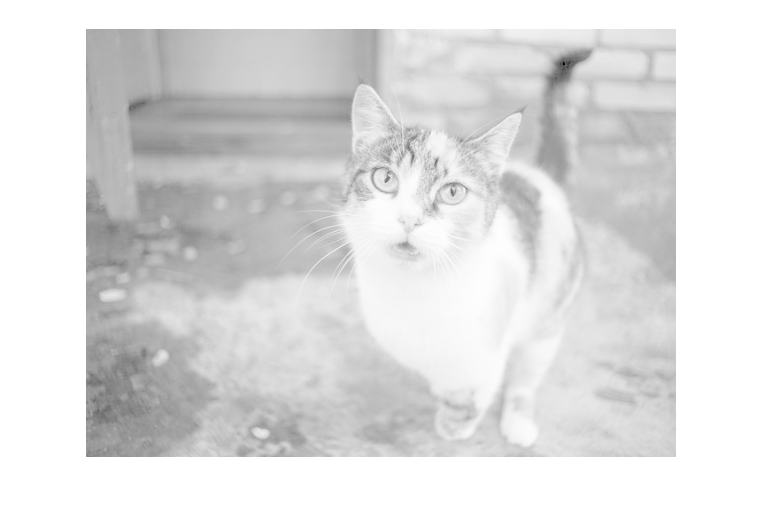
\includegraphics[width=\linewidth]{../../lab02/cat_gamma.png}
		\captionof{figure}{Zwiększenie luminacji}
		\label{fig:cat_gamma}
	\end{center}
	
	\begin{center}
		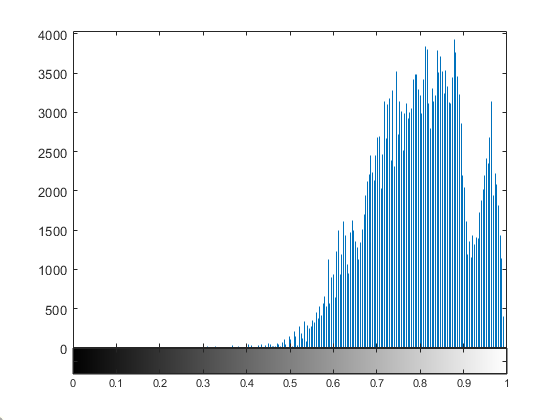
\includegraphics[width=\linewidth]{../../lab02/cat_gamma_hist.png}
		\captionof{figure}{Histogram obrazu ze zwiększoną luminacją.}
		\label{fig:cat_gamma_hist}
	\end{center}
	
	
	\subsection{Wyrównanie Histogramu}
	To przekształcenie polega na zwiększeniu kontrastu poprzez mapowanie odcieni szarości w taki sposób by histogram był jak najbardziej wyrównany.
	
	\begin{center}
	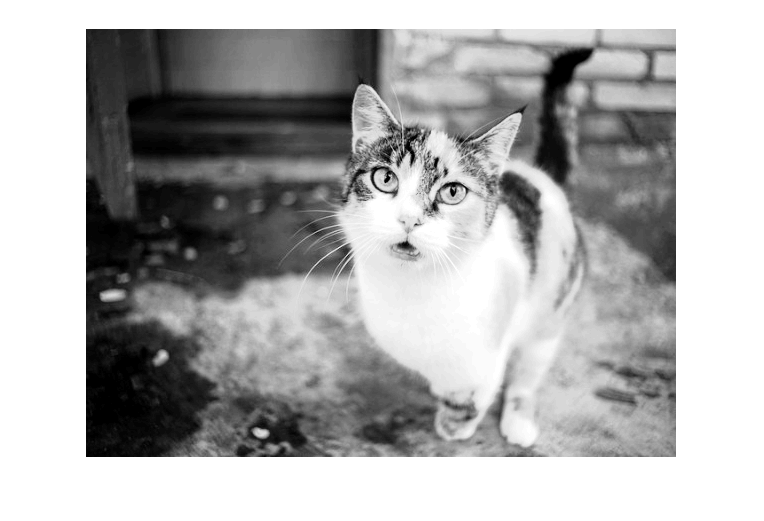
\includegraphics[width=\linewidth]{../../lab02/cat_eq.png}
	\captionof{figure}{Obraz z wyrównanym histogramem}
	\label{fig:cat_eq}
	\end{center}
	
	\begin{center}
		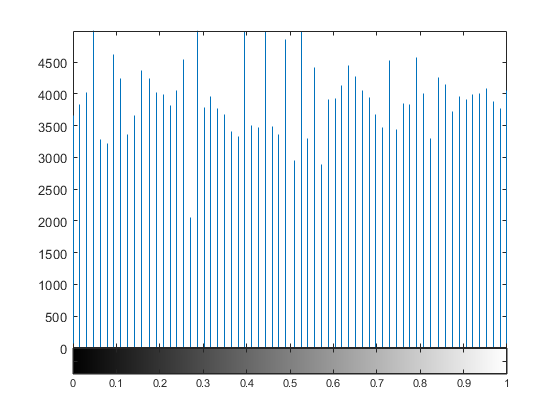
\includegraphics[width=\linewidth]{../../lab02/cat_eq_hist.png}
		\captionof{figure}{Wyrównany histogram}
		\label{fig:cat_eq_hist}
	\end{center}
	
	\begin{center}
		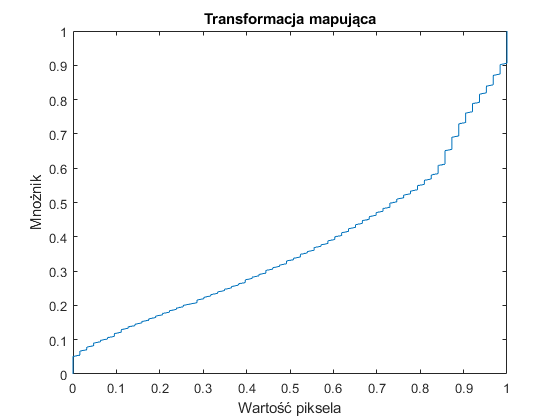
\includegraphics[width=\linewidth]{../../lab02/cat_eq_map.png}
		\label{fig:cat_eq_map}
	\end{center}
	
	
	\section{Laboratorium 3 - Filtrowanie}
	\subsection{Wstęp}
	\begin{center}
		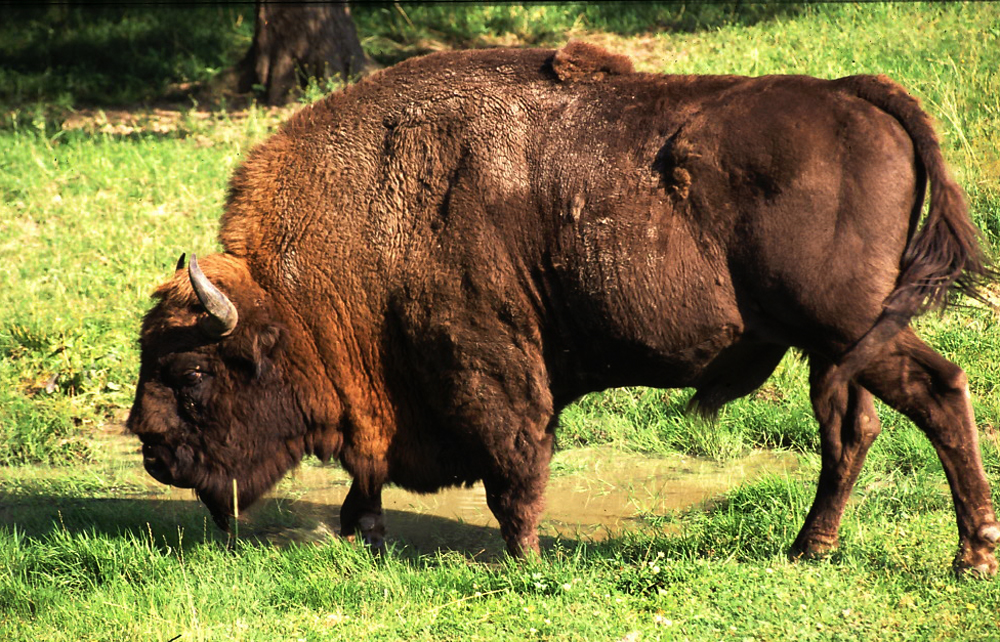
\includegraphics[width=\linewidth]{../../pictures/zubr.jpg}
		\captionof{figure}{Obraz bazowy}
		\label{fig:bison}
	\end{center}
	Na tych laboratoriach mofyfikowaliśmy obrazy poprzez stosowanie różnych filtrów. Wykonując splot jądra (Macierz liczbowa współczynników) z obrazem możemy uzyskać różne efekty.
	
	\paragraph{Filtry dolnoprzepustowe} usuwają elementy o wysokiej częstotliwości np. duże różnice w wartości pikseli. W rezultacie rozmywają obraz.
	
	\paragraph{Filtry górnoprzepustowe} usuwają elementy o niskiej częstotliwości. W rezultacie podkreślają one ostre krawędzie obrazu.
	
	\subsection{Filtr górnoprzepustowy}
	\begin{equation}
	\begin{bmatrix}
	-1 & -1 & -1 \\
	-1 & 9 & -1 \\
	-1 & -1 & -1 
	\end{bmatrix}
	\end{equation}
	\begin{center}
		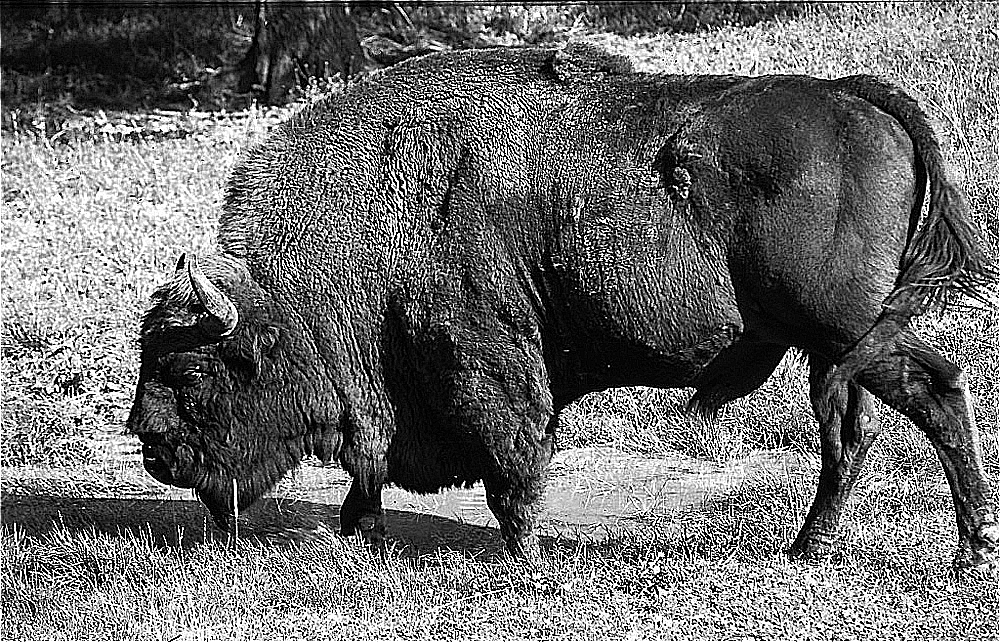
\includegraphics[width=\linewidth]{../../lab03/bison_high-pass.png}
		\captionof{figure}{Rezultat filtru górnoprzepustowego.}
	\end{center}

	\subsection{Rozmycie Gaussowskie - filtr dolnoprzepustowy}
	Dyskretna aproksymacja rozkładu normalnego:
	\begin{equation}
		\left[
			\begin{matrix}
				1 & 2 & 1 \\
				2 & 4 & 2 \\
				1 & 2 & 1 
			\end{matrix}
		\right]
	\end{equation}
	
	\begin{center}
		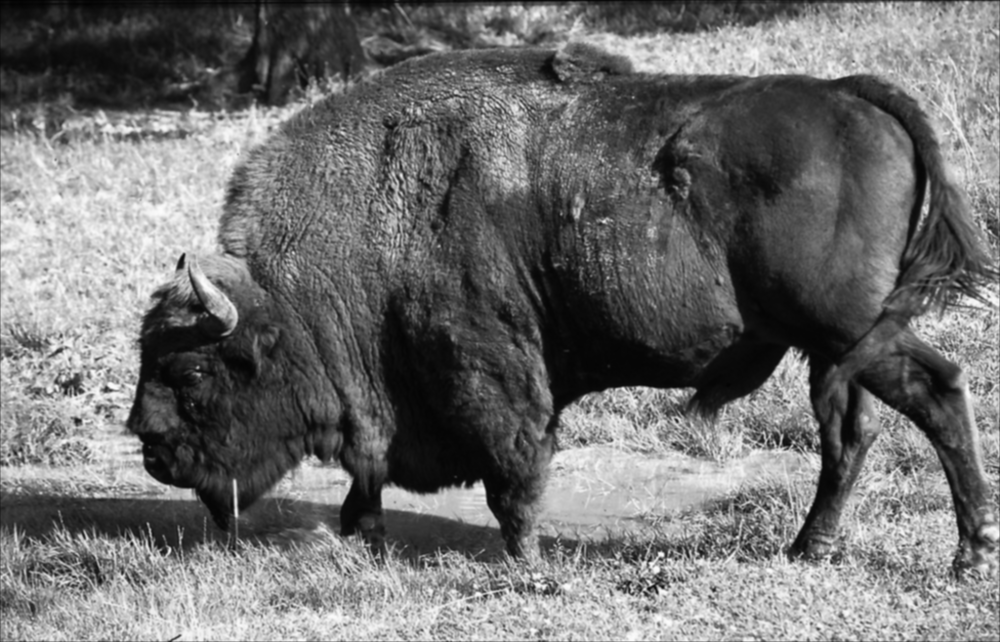
\includegraphics[width=\linewidth]{../../lab03/bison_gauss.png}
		\captionof{figure}{Rezultat rozmycia Gaussowskiego}
		\label{fig:bison_gauss}
	\end{center}
	
	
	\subsection{Średnia Arytmetyczna - filtr dolnoprzepustowy}
	\begin{equation}
	\left[
	\begin{matrix}
	1 & 1 & 1 \\
	1 & 1 & 1 \\
	1 & 1 & 1 
	\end{matrix}
	\right]
	\end{equation}
	
	\begin{center}
		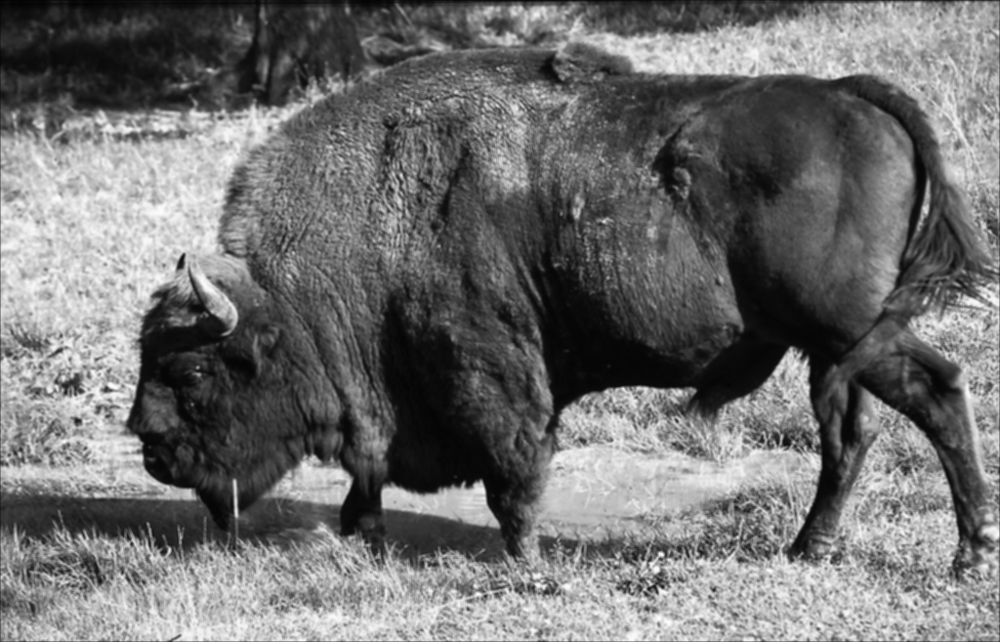
\includegraphics[width=\linewidth]{../../lab03/bison_avg.png}
		\captionof{figure}{Rezultat filtru uśredniającego}
		\label{fig:bison_avg}
	\end{center}

	\subsection{Mediana - filtr dolnoprzepustowy}
	Do wyznaczenia nowej wartości piksela możemy też posłużyć się medianą wartości sąsiednich pikseli. Tutaj użyjemy najbliższych 7 pikseli.
	
	Używając mediany nie tworzymy nowych wartości pikseli, zmniejsza to zbiór obrazu.
	
	\begin{center}
		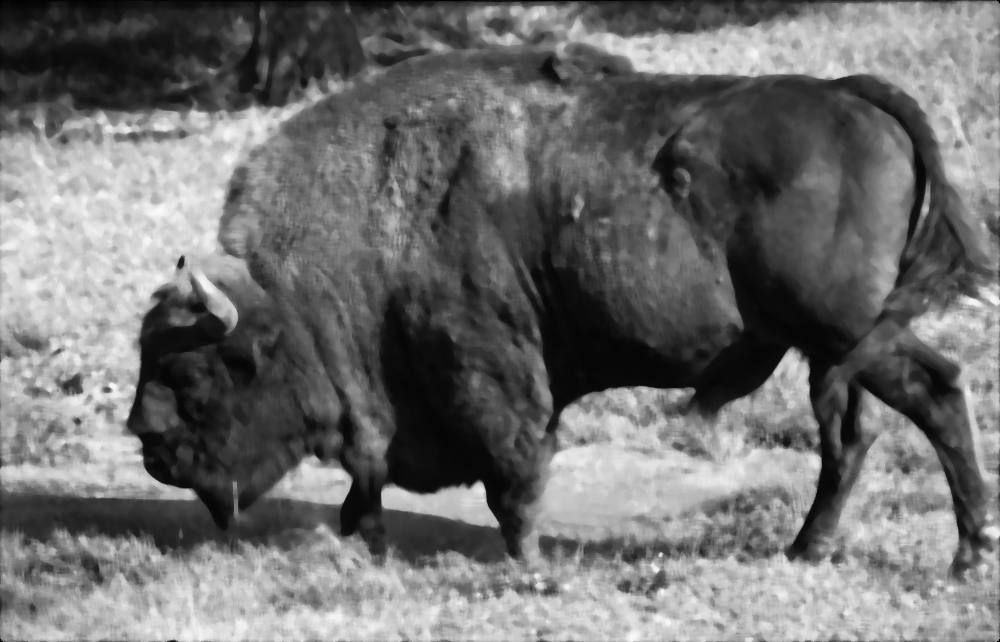
\includegraphics[width=\linewidth]{../../lab03/bison_med.png}
		\captionof{figure}{Rezultat filtru medianowego}
		\label{fig:bison_med}
	\end{center}
	\begin{center}
		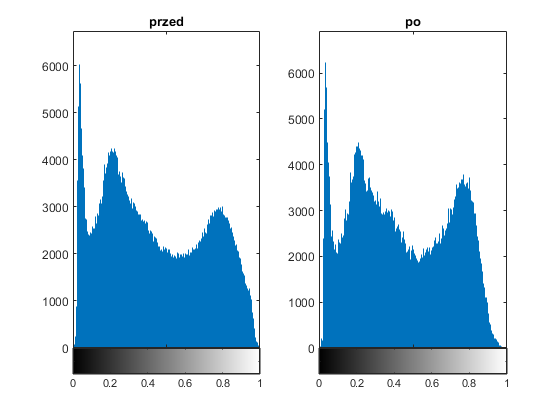
\includegraphics[width=\linewidth]{../../lab03/bison_hist.png}
		\captionof{figure}{Histogramy przed i po filtrze medianowym}
		\label{fig:bison_hist}
	\end{center}
	
	\subsection{Filtr Sobela}
	Filtry wykrywające poziome i pionowe krawędzie.
	\begin{equation}
	\begin{bmatrix}
	1 & 2 & 1 \\
	0 & 0 & 0 \\
	-1 & -2 & -1 
	\end{bmatrix}
	,
	\begin{bmatrix}
	1 & 0 & -1 \\
	2 & 0 & -2 \\
	1 & 0 & -1 
	\end{bmatrix}
	\end{equation}
	
	\begin{center}
		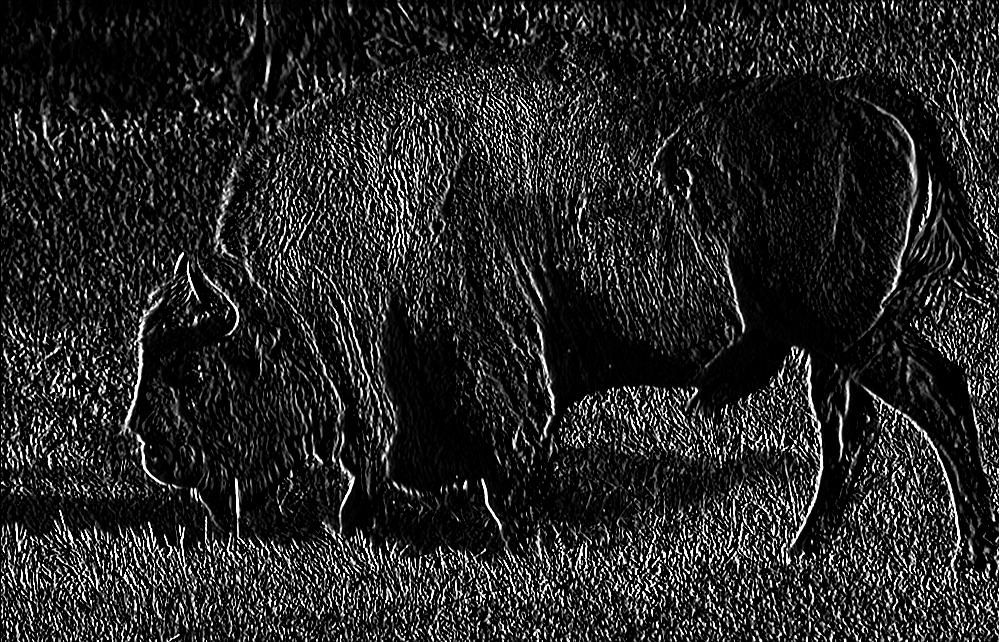
\includegraphics[width=\linewidth]{../../lab03/bison_sobel.png}
		\captionof{figure}{Rezultat filtru Sobel'a}
		\label{fig:bison_sobel}
	\end{center}

	\subsection{Binaryzacja}
	Do binaryzacji obrazu niezbedne jest wybranie progu względem którego będziemy dzielić piksele na dwie kategorie (0,1).
	Do wyznaczenia globalnego progu T wykorzystamy metodę Otsu.
	Do wyznaczenia progu lokalnego skorzystamy z metody adaptacyjnej.
	
	\begin{center}
		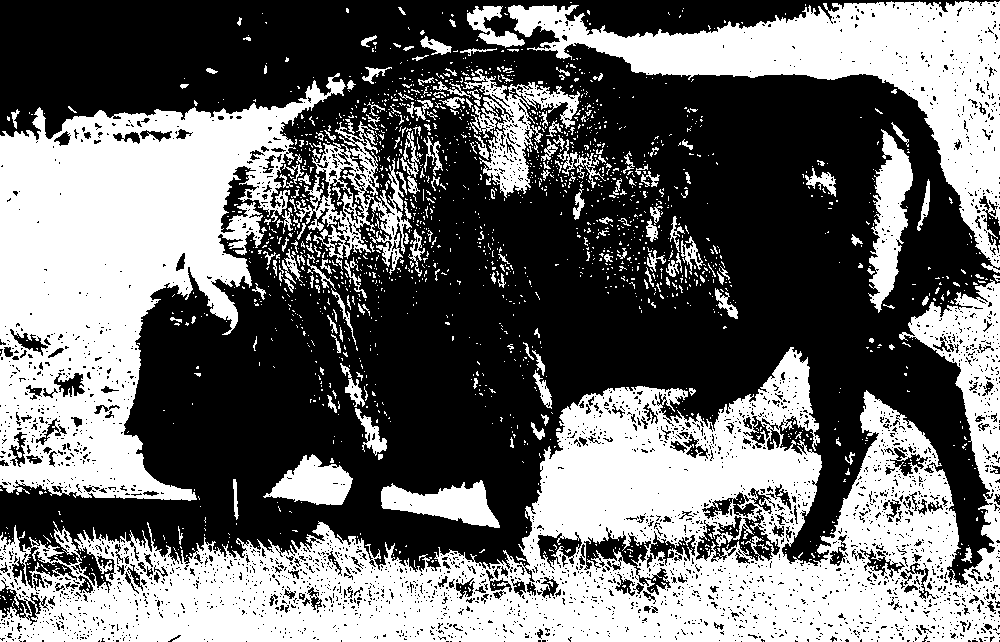
\includegraphics[width=\linewidth]{../../lab03/bison_bin_otsu.png}
		\captionof{figure}{Rezultat binaryzacji. Metoda Otsu, T = 0.4706}
	\end{center}
	\begin{center}
		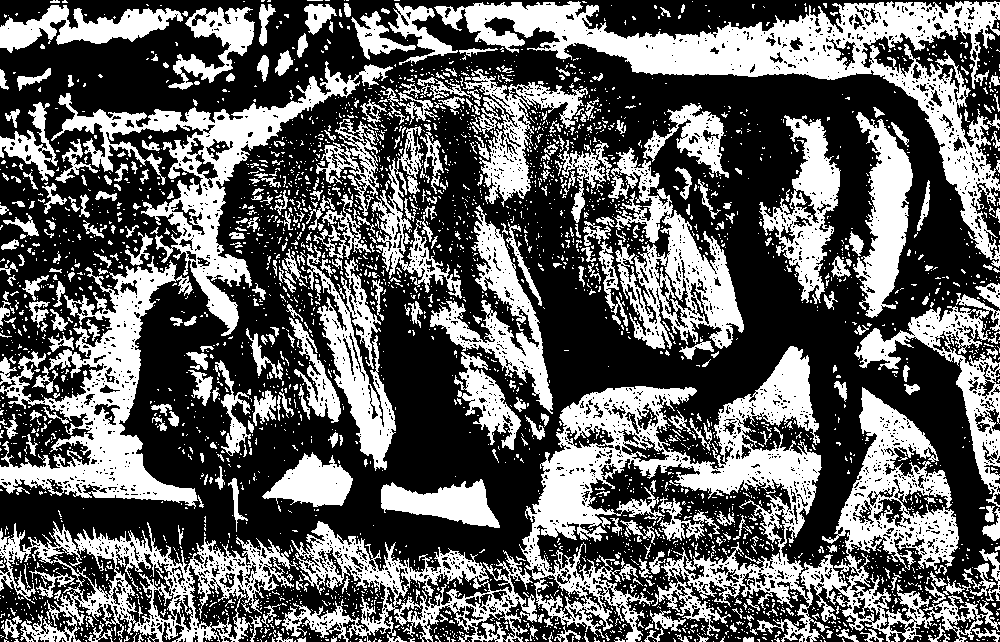
\includegraphics[width=\linewidth]{../../lab03/bison_bin_adaptive.png}
		\captionof{figure}{Rezultat binaryzacji. Metoda adaptacyjna}
	\end{center}
	Dla obrazu binarnego, moda i mediana działają tak samo.

	\subsection{Operacje morfologiczne}
	Czyli takie które zmieniają kształty w obrazie. Wykonuje się je na obrazie binarnym.
	\begin{center}
		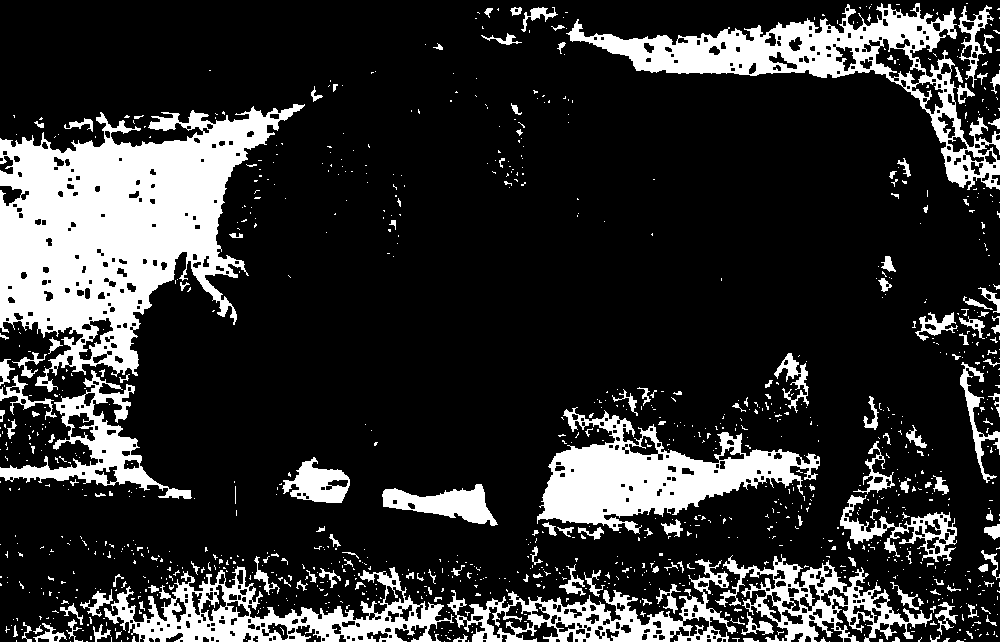
\includegraphics[width=\linewidth]{../../lab03/bison_erode.png}
		\captionof{figure}{Erozja}
	\end{center}
	\begin{center}
		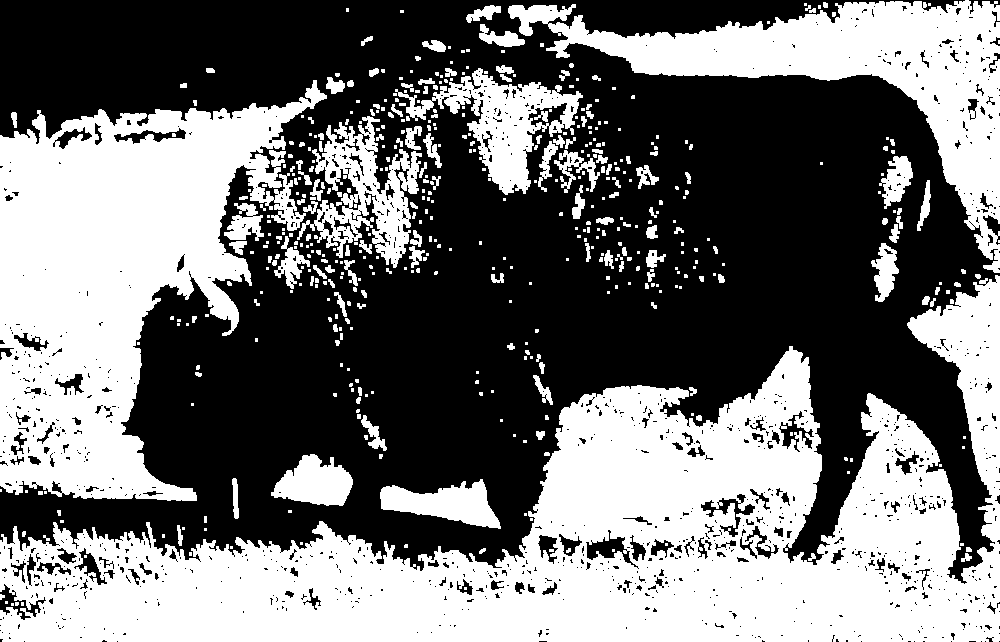
\includegraphics[width=\linewidth]{../../lab03/bison_dilate.png}
		\captionof{figure}{Dylatacja}
	\end{center}
	\begin{center}
		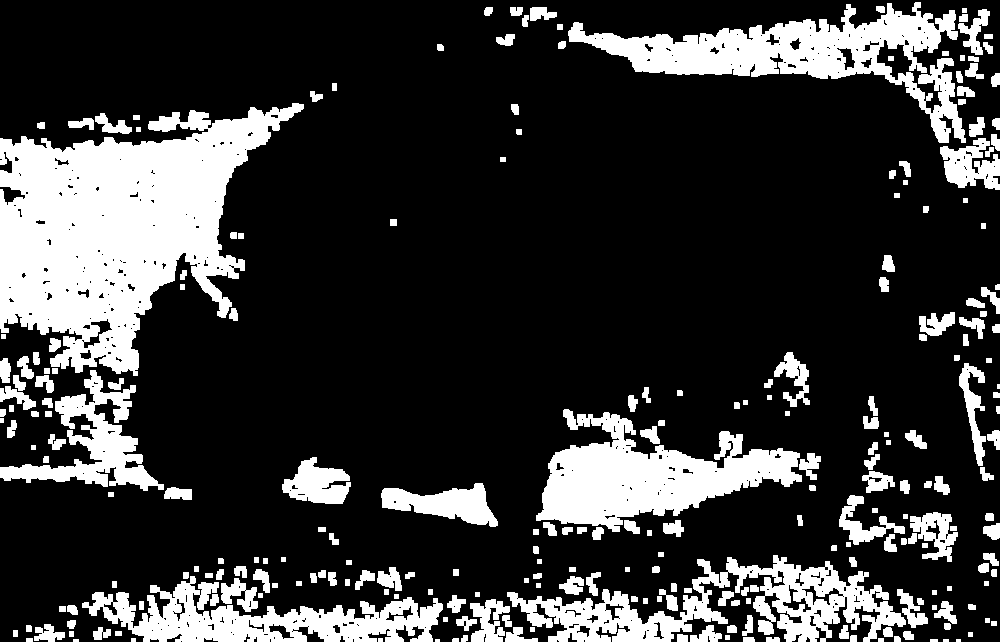
\includegraphics[width=\linewidth]{../../lab03/bison_open.png}
		\captionof{figure}{Erozja + Dylatacja = Otwarcie}
	\end{center}
	\begin{center}
		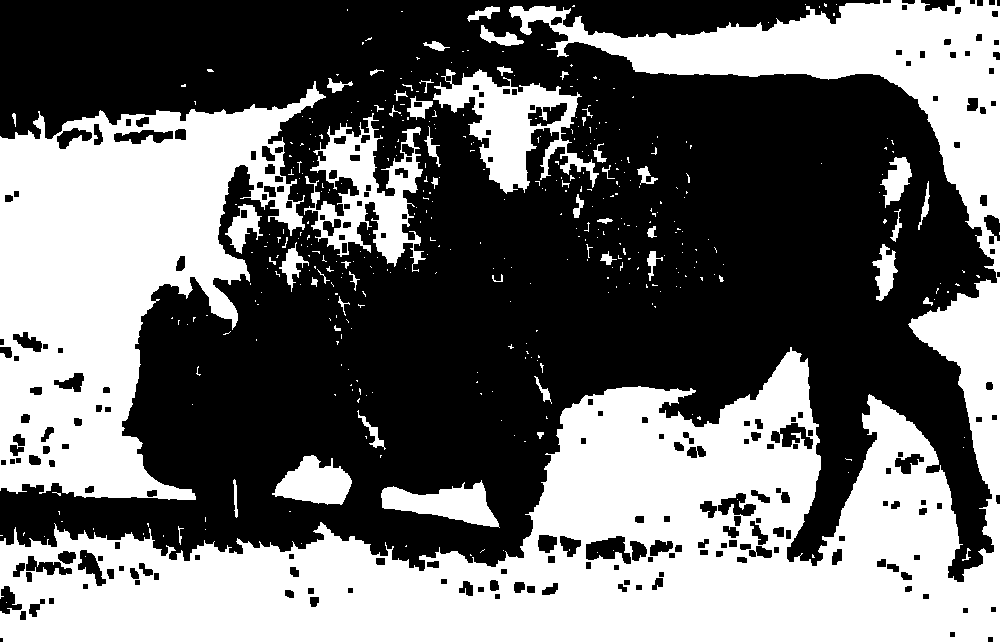
\includegraphics[width=\linewidth]{../../lab03/bison_close.png}
		\captionof{figure}{Dylatacja + Erozja = Zamknięcie}
	\end{center}

	Erozję i dylatację można też wykorzystać do znajdowania krawędzi.
	Wystarczy, że od binarnego obrazu bazowego odejmiemy obraz po erozji. Albo od obrazu po dylatacji odejmiemy binarny obraz bazowy.
	\begin{center}
		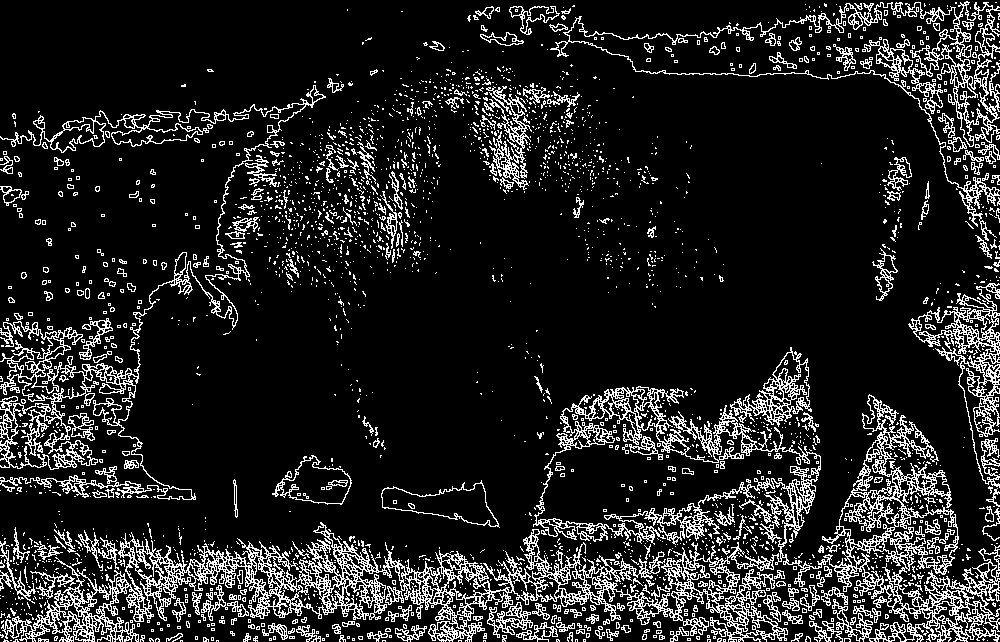
\includegraphics[width=\linewidth]{../../lab03/bison_edge_erode.png}
		\captionof{figure}{Erozja, krawędzie}
	\end{center}
	\begin{center}
		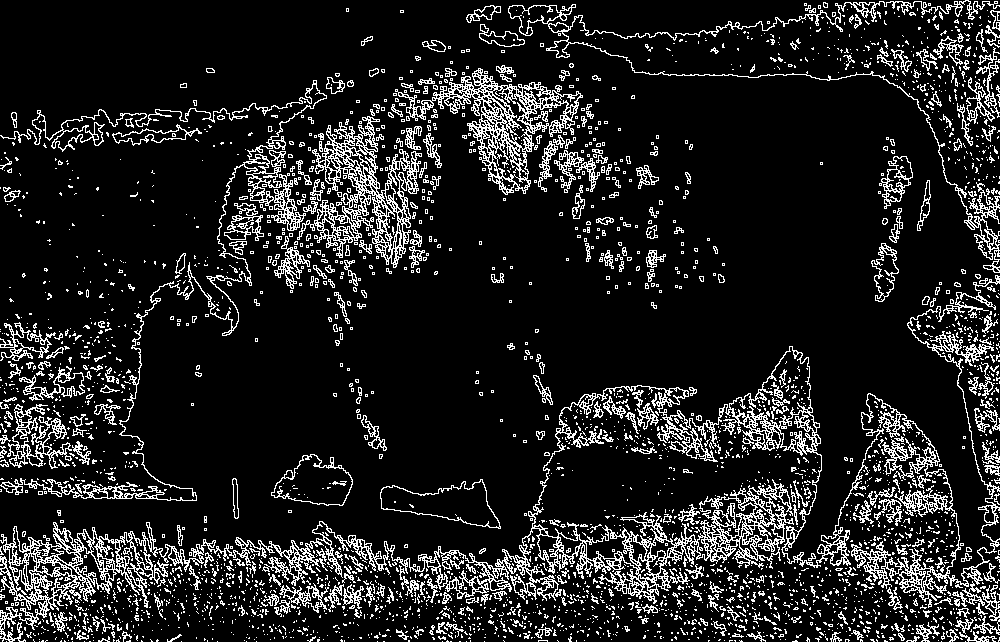
\includegraphics[width=\linewidth]{../../lab03/bison_edge_dilate.png}
		\captionof{figure}{Dylatacja, krawędzie}
	\end{center}

	\subsection{Filtr wykrywający krawędzie}
	\begin{equation}
	\begin{bmatrix}
	-1 & -1 & -1 \\
	-1 & 8 & -1 \\
	-1 & -1 & -1 
	\end{bmatrix}
	\end{equation}
	\begin{center}
		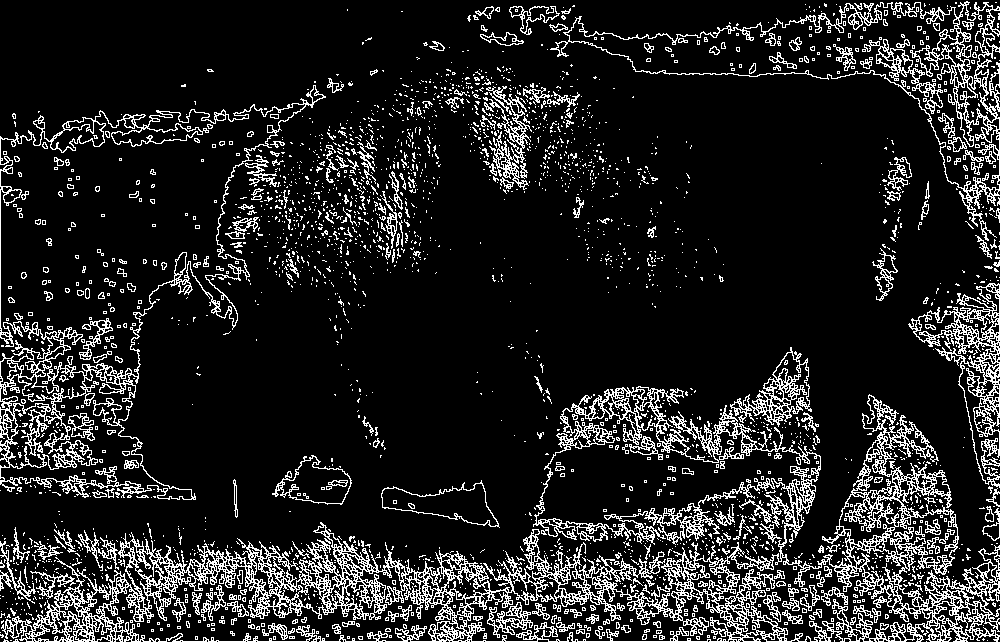
\includegraphics[width=\linewidth]{../../lab03/bison_edge.png}
		\captionof{figure}{Rezultat powyższego filtru.}
	\end{center}

	Przeanalizujmy działanie tego filtru:
	\begin{enumerate}
		\item Gdy natrafi na piksel który nie jest krawędzią(ma taką samą wartość jak sąsiedzi) to jego wartość będzie wynosić 0.
		
		\item Gdy natrafi na piksel który ma chociaż jednego różniącego się sąsiada to jego wartość będzie wynosić 1.
	\end{enumerate}
	W ten prosty sposób jesteśmy w stanie wyznaczyć miejsca w których wartość pikseli się zmienia.
	
	\subsection{Maska}
	Obraz binarny możemy wykorzystać jako maskę i z obrazu bazowego "wyciąć" wykryty przez nas kształt. Wystarczy wykonać iloczyn obrazu binarnego i bazowego.
	\begin{center}
		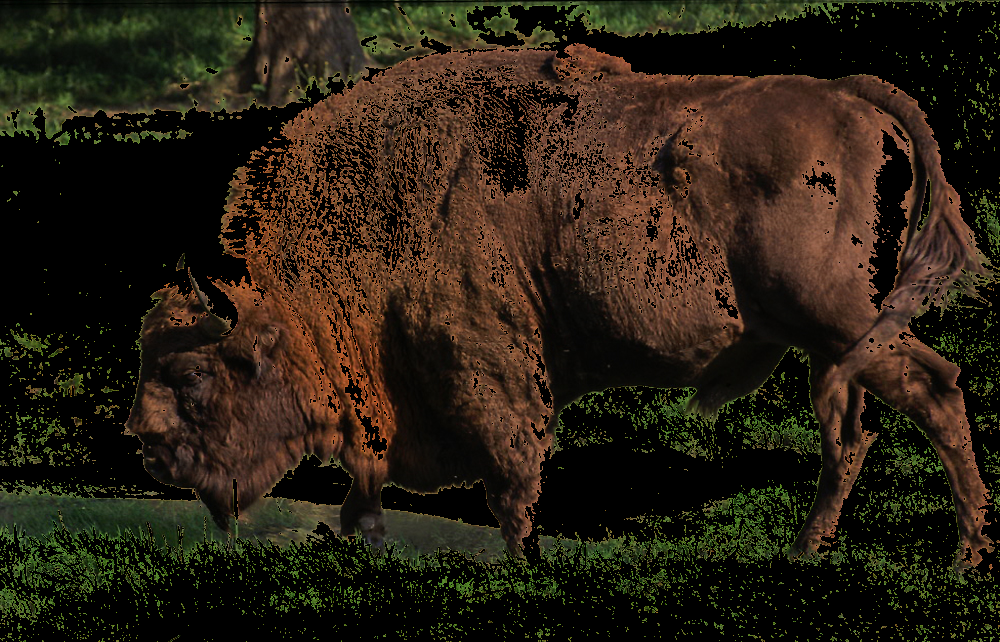
\includegraphics[width=\linewidth]{../../lab03/bison_mask.png}
		\captionof{figure}{Przykład użycia maski}
	\end{center}
	
	\section{Laboratorium 4 - Transformacja Fouriera}
	\begin{center}
		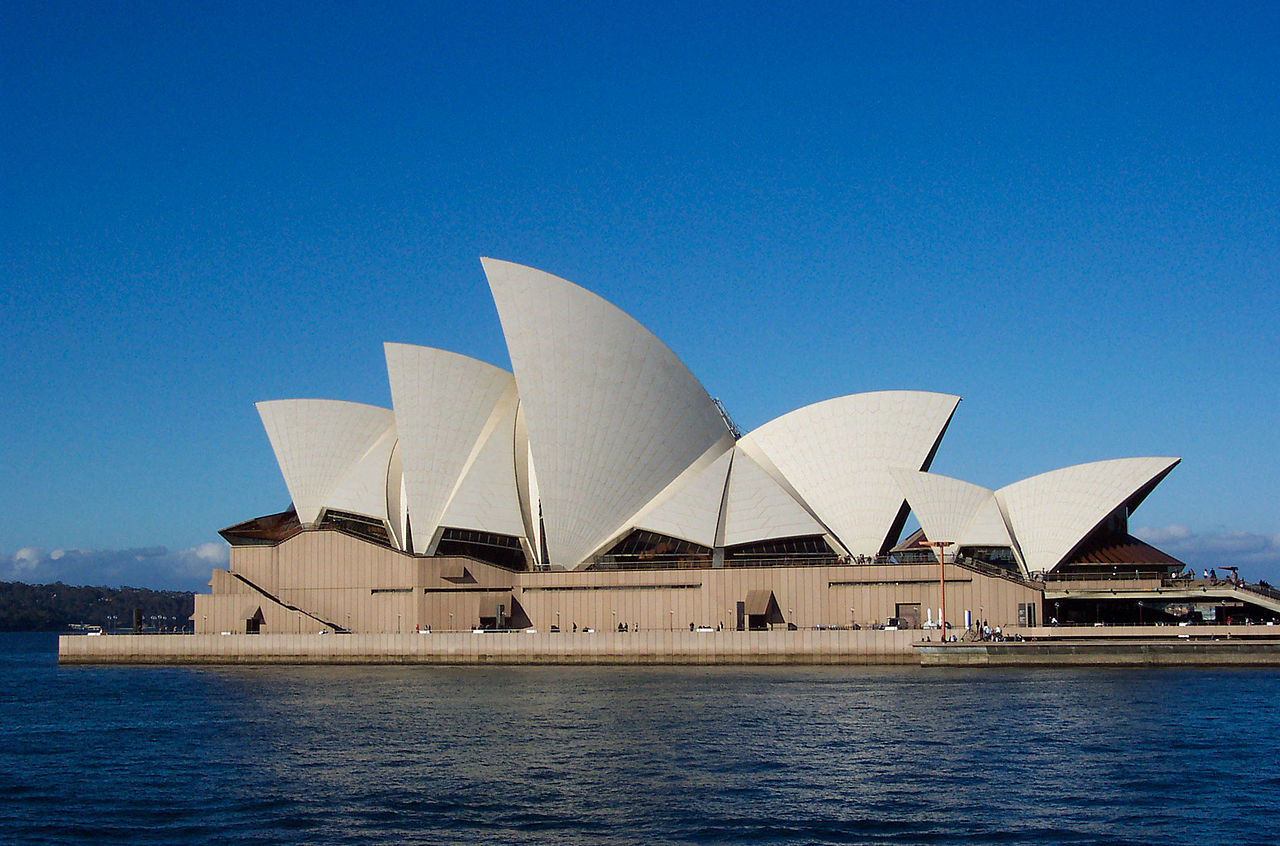
\includegraphics[width=\linewidth]{../../pictures/opera.jpg}
		\captionof{figure}{Obraz bazowy}
	\end{center}
	\subsection{Interpretacja widm}
	\paragraph{Widmo amplitudowe}
	daje nam informację o cechach geometrycznych obrazu. Na poniższym przykładzie poszczególne linie na widmie amplitudowym korespondują z kształtami sklepienia opery.
	\begin{center}
		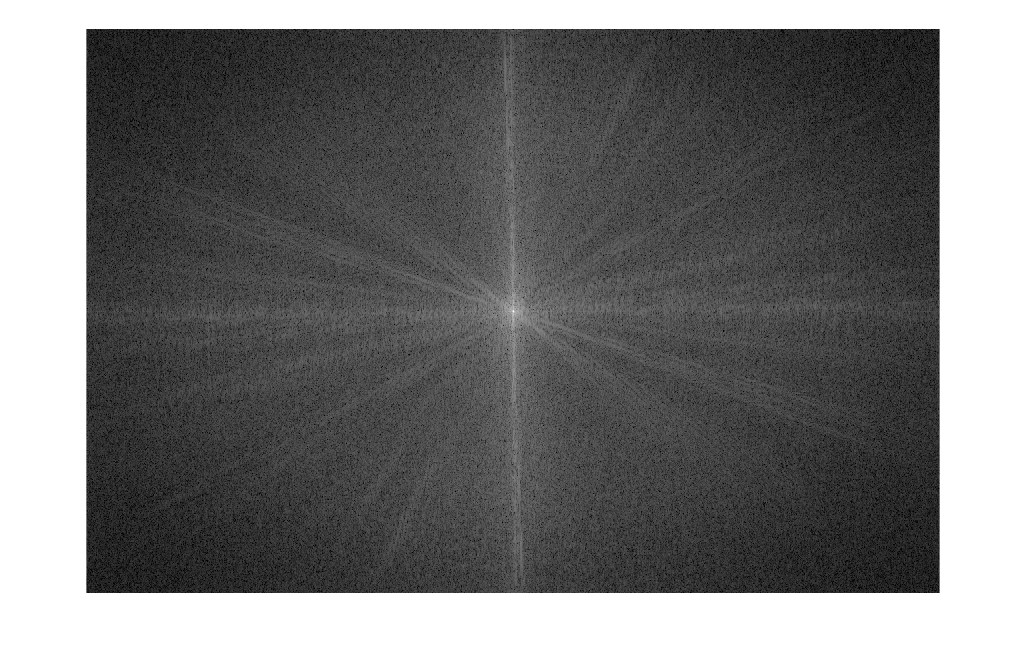
\includegraphics[width=\linewidth]{../../lab04/amplitude_spectrum.png}
		\captionof{figure}{Widmo amplitudowe}
	\end{center}
	\paragraph{Widmo fazowe}
	\begin{center}
		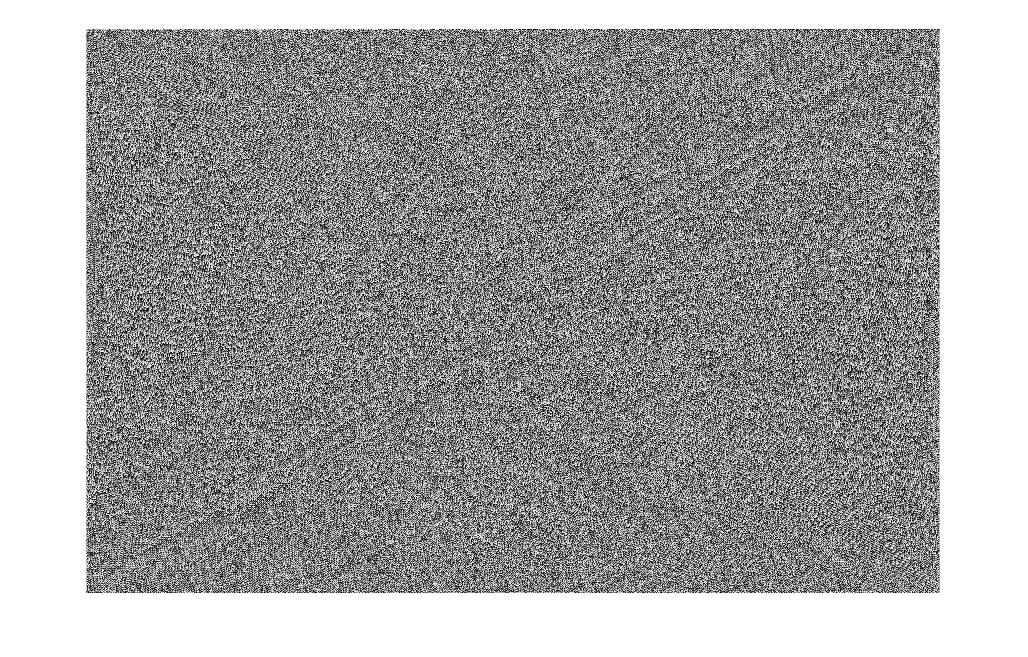
\includegraphics[width=\linewidth]{../../lab04/angle_spectrum.png}
		\captionof{figure}{Widmo fazowe}
	\end{center}
	
	\paragraph{Wykrywanie modyfikacji obrazu}
	Jeżeli w widmie fazowym obrazu występują regularne kształty to znaczy, że obraz bazowy posiada okresowe zakłócenia.
	Może to oznaczać, że obraz był modyfikowany.
	\subsection{Negatyw}
	Zmieniając fazę na przeciwną otrzymujemy negatyw obrazu bazowego.
	\begin{center}
		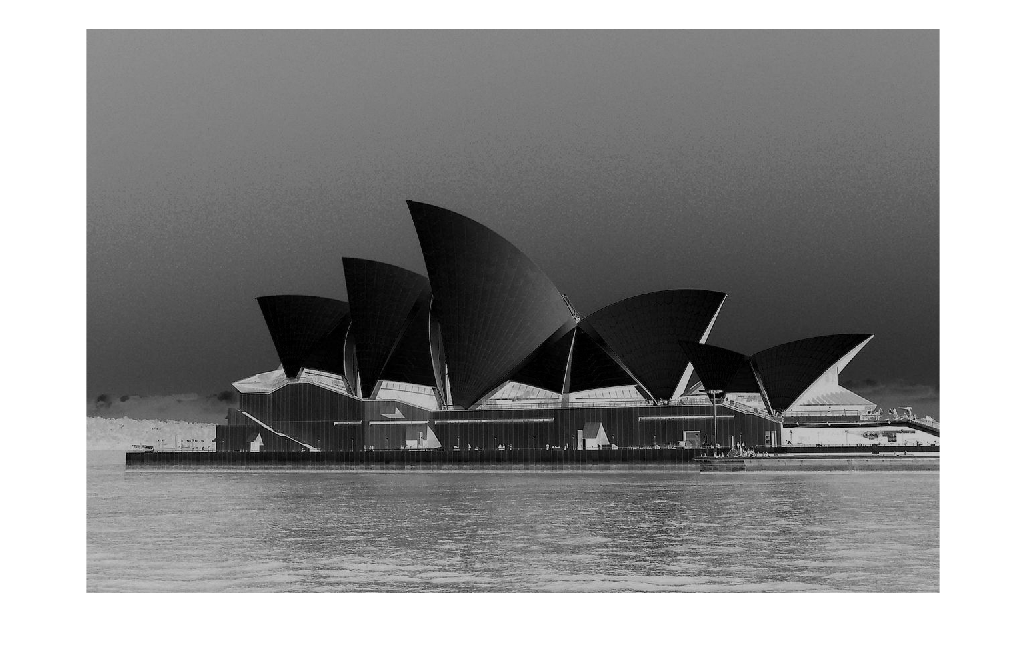
\includegraphics[width=\linewidth]{../../lab04/negative.png}
		\captionof{figure}{Widmo fazowe}
	\end{center}
	
	
	\subsection{Zmiana amplitudy}
	Mnożąc lub potęgując każdy piksel widma amplitudowego możemy rozjaśniać lub przyciemniać obraz bazowy.
	
	
	\subsection{Zaburzenie punktowe}
	Zobaczmy co się stanie gdy wartość jednego piksela zwiększymy do 100 000.
	\begin{center}
		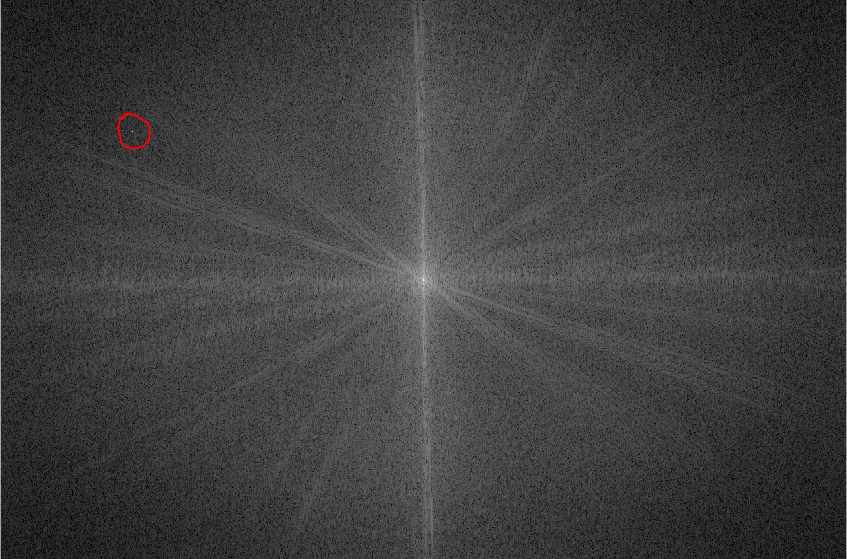
\includegraphics[width=\linewidth]{../../lab04/white_pixel.png}
		\captionof{figure}{Widmo amplitudowe, zmiana jednego piksela}
	\end{center}
	\begin{center}
		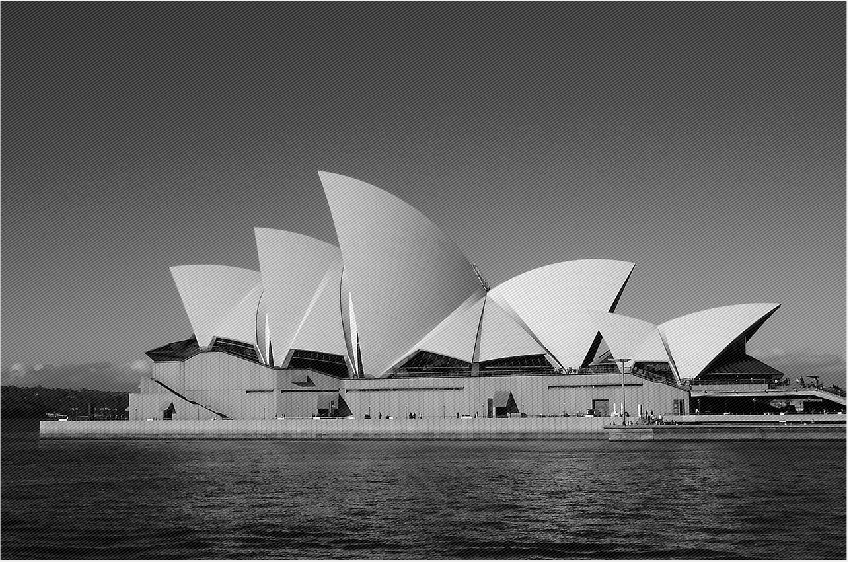
\includegraphics[width=\linewidth]{../../lab04/white_pixel_effect.png}
		\captionof{figure}{Obraz bazowy, zmiana jednego piksela}
	\end{center}
	Spowodowało to pojawienie się okresowego zaburzenia na obrazie bazowym w kształcie ukośnych linii.
	Piksele widma nie są powiązane bezpośrednio z pikselami obrazu bazowego.

	
	\subsection{Filtr dolnoprzepustowy}
		\begin{center}
			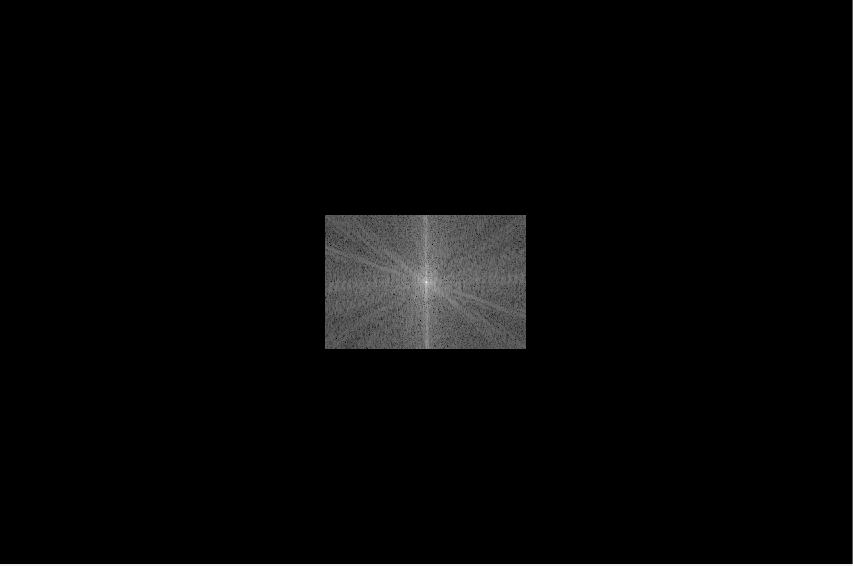
\includegraphics[width=\linewidth]{../../lab04/mask.png}
			\captionof{figure}{Widmo amplitudowe z maską}
		\end{center}
		\begin{center}
			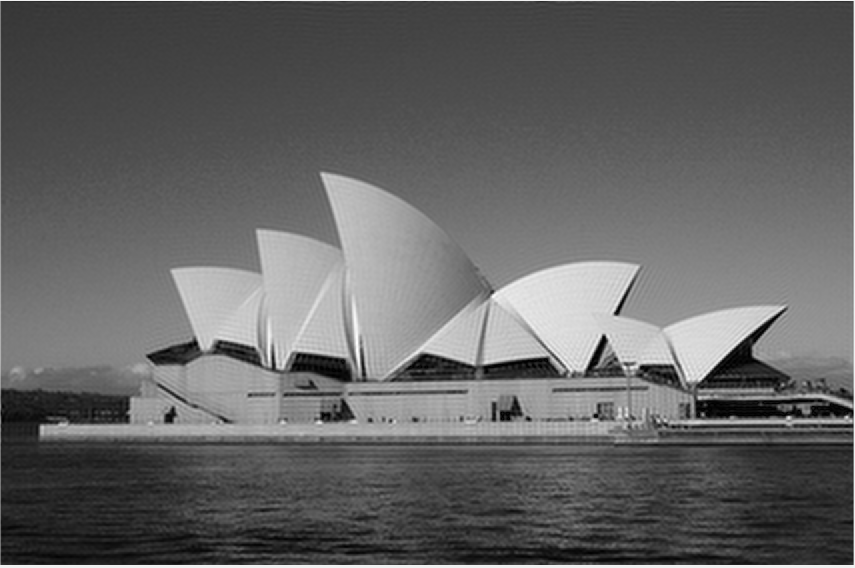
\includegraphics[width=\linewidth]{../../lab04/mask_applied.png}
			\captionof{figure}{Rezultat zastosowania maski na widmie amplitudowym}
		\end{center}
	Usunięcie sygnałów o małych częstotliwościach z widma amplitudowego, spowodowało usunięcie szumu z obrazu bazowego. Usunięcie szumu bardzo ułatwia dalszą analizę obrazu innymi algorytmami mimo, że dla ludzkiego oka może wydawać się rozmazane.
	\paragraph{Kompresja}
	Zredukowaliśmy rozmiar widma obrazu do $\frac{300 \cdot 200}{846 \cdot 1280} = 5.54\%$ oryginału, a mimo to nadal jest on dla nas czytelny. FFT sprawdza się bardzo dobrze w algorytmach kompresji stratnej.
	
\end{document}